%----------------------------------------------------------------------------------------------------
\section{Data analysis}
\label{sec:cni_anal}

\> nuclear modulus: anchored to $90\un{m}$ data at $|t| > 0.2\un{GeV^2}$

\> with the presented data not possible to distinguish between different models/assumptions above $\Rightarrow$ {\bf conditional} determination of parameters of interest
\>> $\rho$
\>> total cross-section and $B$ with Coulomb separated


\> generalised $\chi^2$ fits (covariance matrix contained all relevant contributions: statistical, normalisation and misalignment), full formula??, fits driven by Minuit

\> extensive MC tests (input: phenomenological models as well as data fits)
\>> check for bias: only small
\>> understanding/evaluation of the method response to statistical and systematic uncertainties

\> results ($\rho$, $\sigma_{\rm tot}$, $B^{\rm N}(0)$, ...)
\>> for the model choices above -- keeping phase parameters fixed at their central values from Vojt\v ech
\>> for peripheral-phase parameters being varied within their uncertainties $\Rightarrow$ uncertainty band

\> question: do we want to present a single-value result for $\rho$ (combined from fits under different models) ??

\> discuss the new value of $\sigma_{\rm tot}$ in comparison to our previous measurement \cite{prl111}; values compatible; remind in what is the new measurement better ??

\> reference to Fig.~\ref{fig:rho_s}

\> RMS of b for the final fits??

\begin{figure*}
\begin{center}
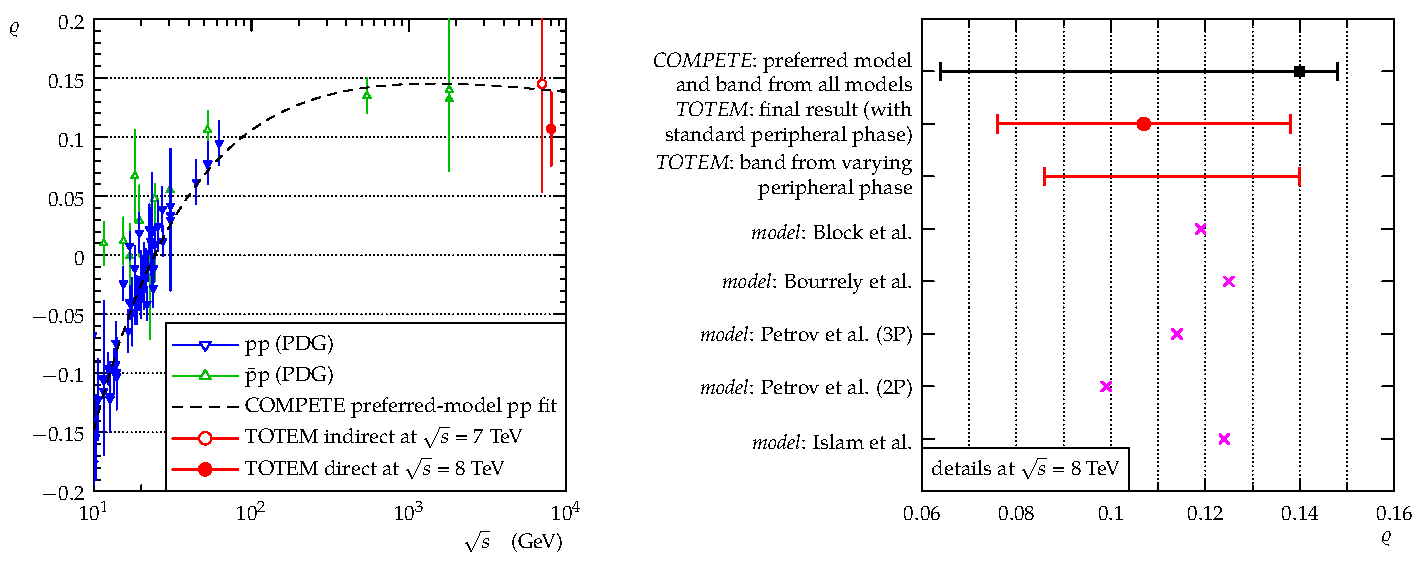
\includegraphics[width=16cm]{fig/rho_s.pdf}
\vskip-3mm
\caption{$\rho$ as a function of $s$.}
\label{fig:rho_s}
\end{center}
\end{figure*}

\> figure for $\sigma_{\rm tot}$ result ?? 
